\section{Part 2: Examination of the Real Data NewData3}

\begin{taskbox}[Tasks]
The same steps as for NewData1 (Questions 1 to 6 of the previous section) are carried out for the second selected recording.
\end{taskbox}

\subsection*{Questions 1 and 2: Observation and identification of the artifact pattern}

The NewData3 recording also has 21 channels and the interval from zero to five seconds. Three slow transients with a large amplitude are seen in the frontal channels at about one, two and a half, and four and a half seconds. There is also localized fast activity in T4. Through the ICA examination, these two patterns led to two independent sets of evidence; large amplitude alone was not made the basis of removal.

\begin{figure}[H]
\centering
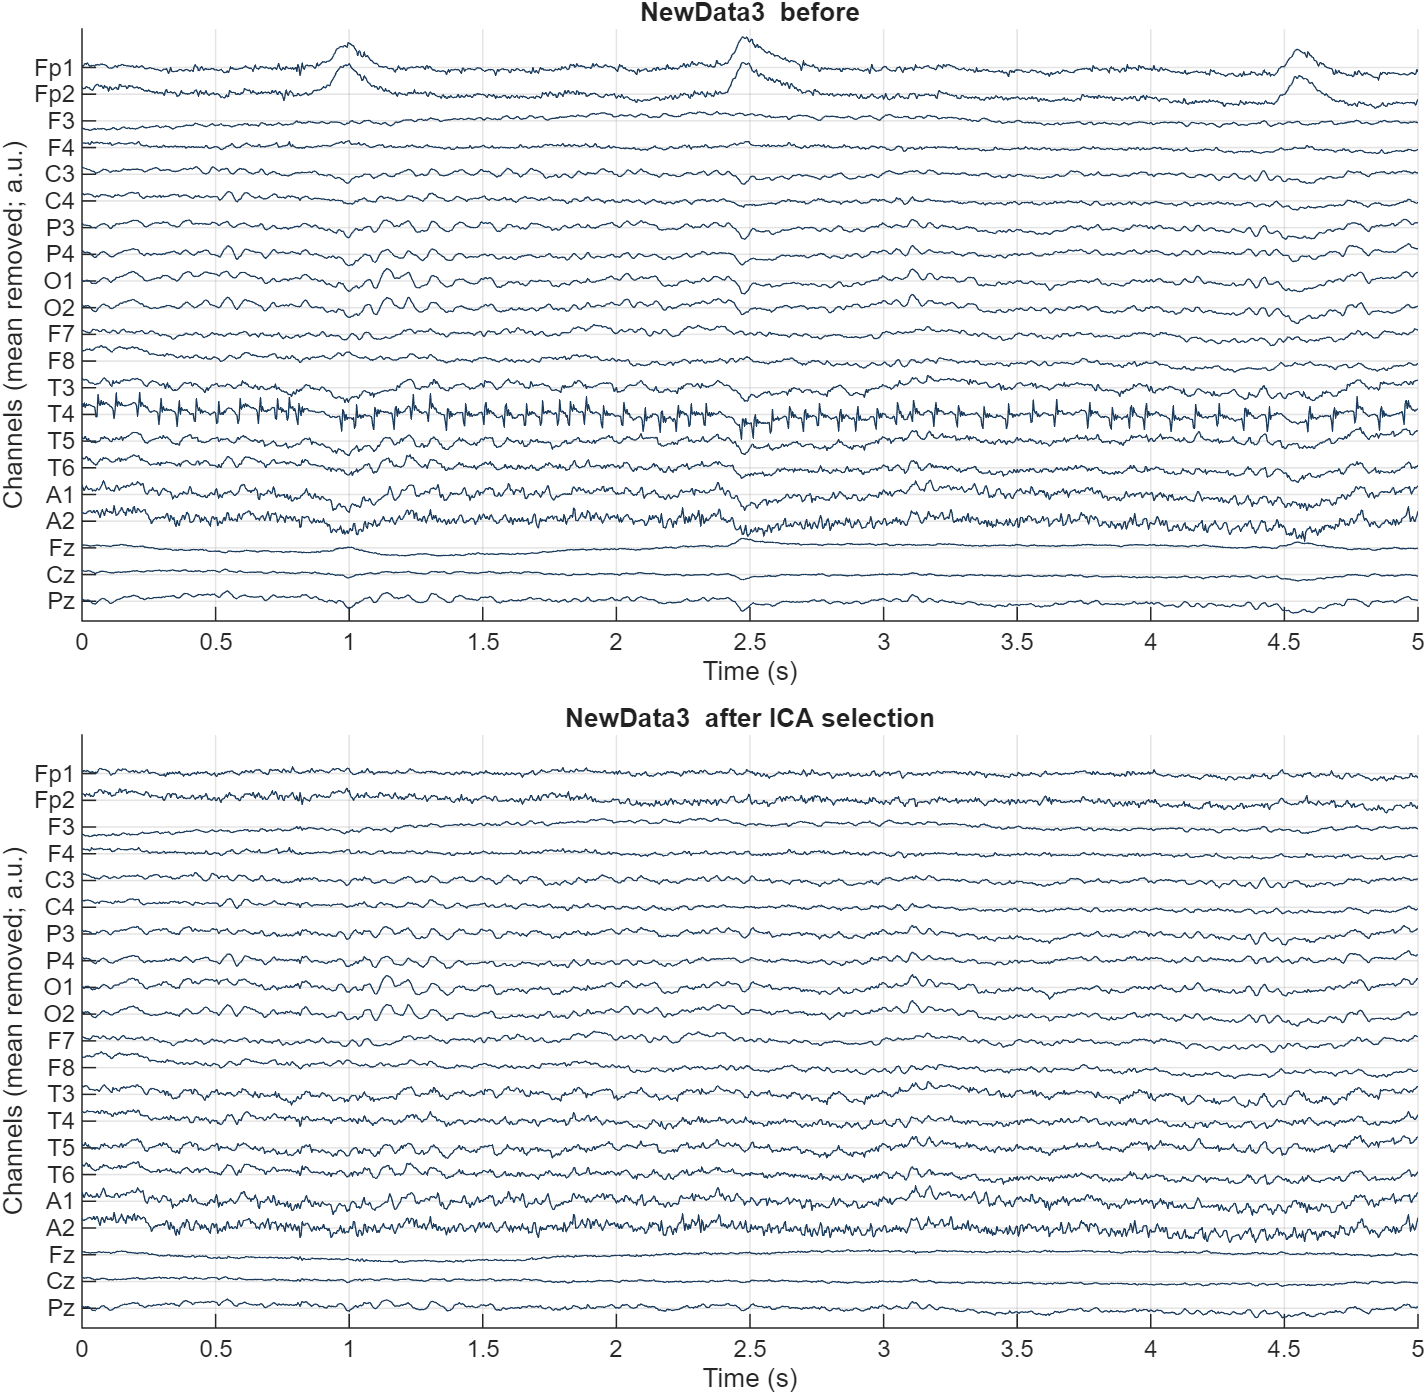
\includegraphics[width=0.85\textwidth,height=0.72\textheight,keepaspectratio]{fig13_newdata3_before_after.png}
\caption{All channels of NewData3 before and after removing IC1 and IC8; common scale, showing the reduction of the frontal transients and of the T4 contamination.}
\label{fig:nd3}
\end{figure}

\subsection*{Selection of components in NewData3}
\subsection*{Questions 3 and 4: Separation and evidence for the components}

The numerical rank was 21, and $A$ and $W$ of size $21\times21$ and $S$ of size $21\times1251$ were obtained. Figures~29 to~31 show the time course, the PSD and the spatial pattern of all components. The two components below had the clearer evidence for tentative removal.

\begin{center}
\begin{tabularx}{\textwidth}{@{}c>{\raggedright\arraybackslash}X>{\raggedright\arraybackslash}X>{\raggedright\arraybackslash}X@{}}
\toprule
\textbf{Component} & \textbf{Temporal and spectral evidence} & \textbf{Spatial evidence} & \textbf{Decision}\\
\midrule
IC1 & Three slow transients; LF $\approx 0.816$ & Frontal share $\approx 0.640$ & Removed as probable blink-like\\
IC8 & HF $\approx 0.805$; lag1 $\approx 0.071$ & Squared-weight concentration $\approx 0.971$ on T4 & Removed as localized high-frequency contamination\\
\bottomrule
\end{tabularx}
\end{center}

In IC1, the coincidence of slow transients, the dominance of low power and a bilateral frontal propagation is consistent with a probable eye blink. In IC8, a broad high-frequency spectrum, a low correlation of adjacent samples and a very strong concentration in T4 support a localized contamination. The peak of IC8 at about 65.4~Hz does not mean a narrow-band linear 65~Hz interference; its spectrum is broad. The exact electrode or muscle origin cannot be determined without independent evidence.

Ambiguous components, including IC14, IC20 and IC21, which have a higher high-frequency share, were kept. In particular, an HF of about 0.619 in IC21 raises the possibility of residual noise, but the spatial dispersion and the absence of specific evidence prevented its definite removal. In epileptic data, a high HF or a sharp event alone is not a sufficient basis for removal.

\subsection*{Question 5: Desired sources and the reconstruction}

\begin{lstlisting}[language=Matlab]
RejectedSources = [1 8];
SelSources = [2 3 4 5 6 7 9 10 11 12 13 14 15 16 17 18 19 20 21];
X_den = A(:,SelSources)*S(SelSources,:) + channelMean;
\end{lstlisting}

In this recording, the back-mapping was carried out with the 19 remaining components. The removal of the two components was justified by two distinct sets of temporal, spectral and spatial evidence; the number of removals is not in itself a quality criterion.

The reduction of low power with the removal of the blink-like component, and the reduction of high power with the removal of the T4 contamination, are consistent with each other. However, the energy ratio of 33.53 percent is neither the percentage of real noise removed nor a measure of the clinical information preserved. The selections are defensible with respect to the available evidence, but the possibility of residual contamination exists. Repeating the selection step with more removals, without independent evidence, is not justified.

\subsection*{Question 6: Evaluation of the NewData3 reconstruction}

\begin{figure}[H]
\centering
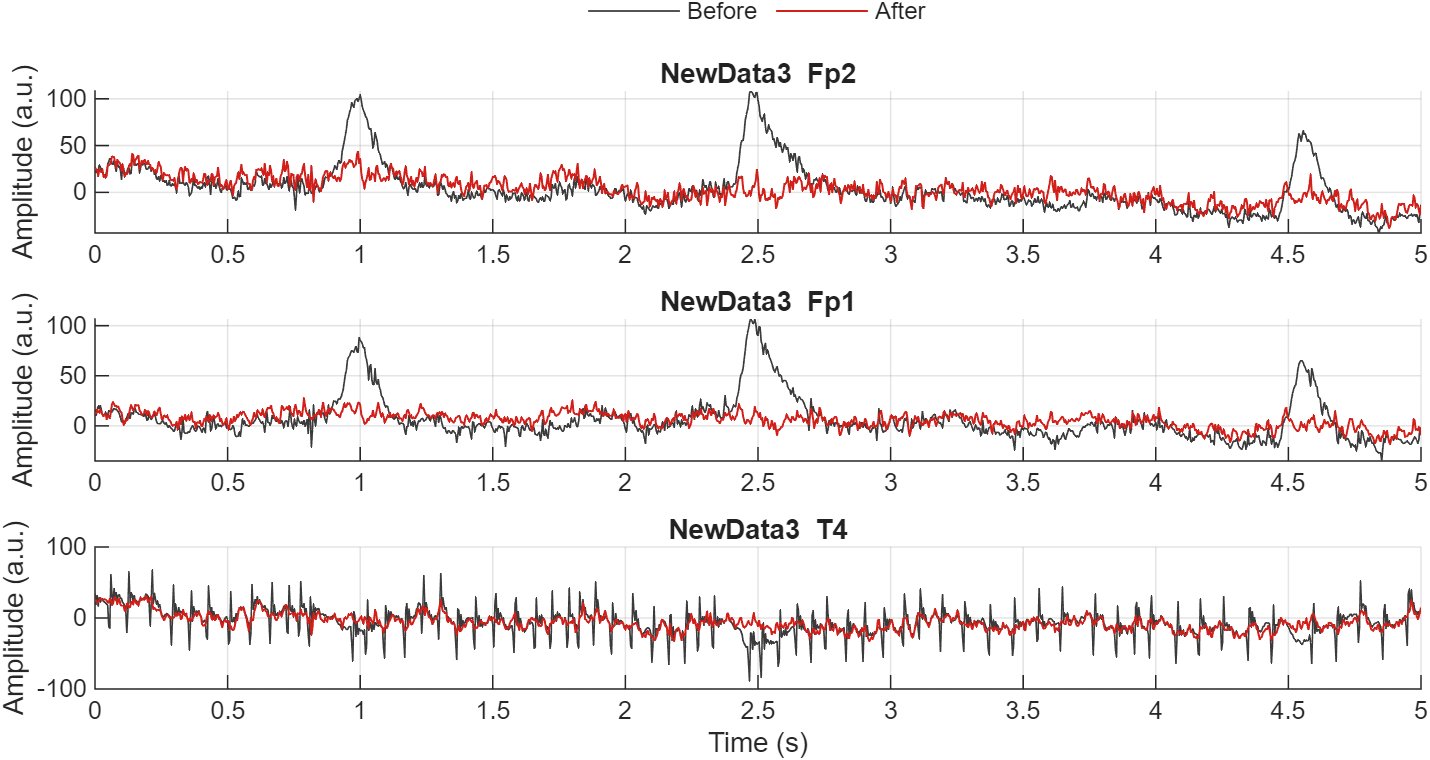
\includegraphics[width=0.9\textwidth]{fig14_newdata3_channels.png}
\caption{Before and after in Fp2, Fp1 and T4; the amplitude of the frontal slow transients and of the localized fast activity has decreased.}
\label{fig:nd3ch}
\end{figure}

\begin{figure}[H]
\centering
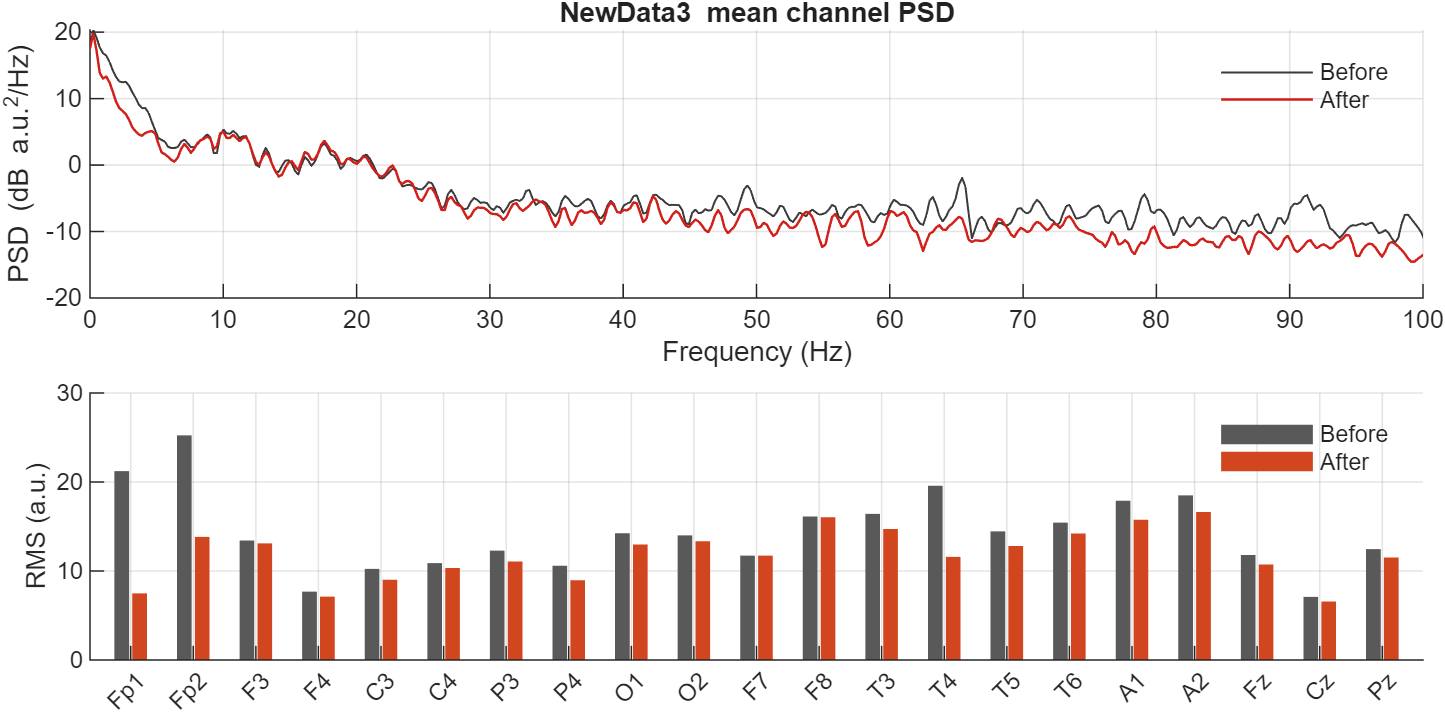
\includegraphics[width=0.9\textwidth]{fig15_newdata3_psd_rms.png}
\caption{Mean PSD and RMS of the channels in NewData3; the simultaneous reduction of low and high power is consistent with the two removed components.}
\label{fig:nd3psd}
\end{figure}

\begin{center}
\begin{tabular}{@{}lc@{}}
\toprule
\textbf{Index} & \textbf{Result}\\
\midrule
Energy ratio of the removed contribution & 0.335279\\
Reduction of the 30--100~Hz power & 2.2695 dB\\
Reduction of the 0.5--4~Hz power & 3.8076 dB\\
Median channel correlation & 0.909780\\
\bottomrule
\end{tabular}
\end{center}
